% ****** Start of file apssamp.tex ******
%
%   This file is part of the APS files in the REVTeX 4.1 distribution.
%   Version 4.1r of REVTeX, August 2010
%
%   Copyright (c) 2009, 2010 The American Physical Society.
%
%   See the REVTeX 4 README file for restrictions and more information.
%
% TeX'ing this file requires that you have AMS-LaTeX 2.0 installed
% as well as the rest of the prerequisites for REVTeX 4.1
%
% See the REVTeX 4 README file
% It also requires running BibTeX. The commands are as follows:
%
%  1)  latex apssamp.tex
%  2)  bibtex apssamp
%  3)  latex apssamp.tex
%  4)  latex apssamp.tex
%
\documentclass[%
 reprint,
nofootinbib,
%superscriptaddress,
%groupedaddress,
%unsortedaddress,
%runinaddress,
%frontmatterverbose,
%preprint,
%showpacs,preprintnumbers,
%nofootinbib,
%nobibnotes,
%bibnotes,
aps,
%pra,
%prb,
%rmp,
%prstab,
%prstper,
%floatfix,
]{revtex4-1}

\usepackage[utf8]{inputenc}
\usepackage[english]{babel}
\usepackage{dsfont}
\usepackage{amsmath}
\usepackage{ mathrsfs }
\usepackage{amssymb}
\usepackage{graphicx}% Include figure files
\usepackage{dcolumn}% Align table columns on decimal point
\usepackage{bm}% bold math
\usepackage{amsmath}
\usepackage{varioref}
\usepackage{booktabs}
\usepackage[bottom]{footmisc}

\usepackage{physics}

\usepackage{algpseudocode}
\usepackage{listings}

\usepackage{booktabs}

\usepackage{tikz}

\newcommand{\RN}[1]{%
  \textup{\uppercase\expandafter{\romannumeral#1}}%
}


\newcolumntype{C}{>{$}c<{$}}
\AtBeginDocument{
\heavyrulewidth=.08em
\lightrulewidth=.05em
\cmidrulewidth=.03em
\belowrulesep=.65ex
\belowbottomsep=0pt
\aboverulesep=.4ex
\abovetopsep=0pt
\cmidrulesep=\doublerulesep
\cmidrulekern=.5em
\defaultaddspace=.5em
}

%\usepackage{hyperref}% add hypertext capabilities
%\usepackage[mathlines]{lineno}% Enable numbering of text and display math
%\linenumbers\relax % Commence numbering lines

%\usepackage[showframe,%Uncomment any one of the following lines to test
%%scale=0.7, marginratio={1:1, 2:3}, ignoreall,% default settings
%%text={7in,10in},centering,
%%margin=1.5in,
%%total={6.5in,8.75in}, top=1.2in, left=0.9in, includefoot,
%%height=10in,a5paper,hmargin={3cm,0.8in},
%]{geometry}

\begin{document}

%\preprint{APS/123-QED}

\title{Variational Monte Carlo of electrons in a quantum dot}% Force line breaks with \\

\author{Cecilie Glittum}\homepage{http://www.github.uio.no/cecilgl/FYS4150}
\author{Ivar Svalheim Haugerud}\homepage{http://www.github.uio.no/ivarsh/FYS4150}

\affiliation{%
 Department of Physics, University of Oslo
}%


\date{\today}% It is always \today, today,
             %  but any date may be explicitly specified

\begin{abstract}
  The Monte Carlo based algorithm, Metropolis, is used together with the variational method to study the ground state of two interacting electrons in a three dimensional harmonic oscillator potential. We begin by studying the equilibration and acceptance rate of the Metropolis algorithm, finding that around $10^5$ Monte Carlo cycles are needed to reach equilibrium. We continue by studying the ground state energy with two different trial wave functions, where only one of them takes the electron-electron interaction into account. The energies of each wave function is minimized with respect to their variational parameters. We find that the trial wave function taking the interaction into account produces the best upper bound of the ground state energy, with an energy of $3.73(1)$ a.u, compared to the analytical value of $3.558$ a.u. The mean distance between the two electrons increase as the characteristic frequency of the potential is decreased, for the interacting Hamiltonian the electrons are always further apart, with a larger energy, than with the non-interacting Hamiltonian.
  The virial theorem is then tested for the interacting and noninteracting case. Where we find that the virial theorem is $\ev{T} = \ev{V}$ without the interaction, but deviates as a function of $\omega$ when the interaction is taken into account. We find that the deviation is due to different terms of the potential energy dominating for different $\omega$, where the repulsion dominates for small $\omega$, but decreases exponentially as $\omega$ increases.
\end{abstract}
\maketitle


\section{Introduction}
The quantum dot (QD) is a hot topic of resarch. Because their highly tunable properties QDs are of wide interest. Potential applications include transistors, solar cells, LEDs, diode lasers, quantum computing, and medical imaging \cite{Q_DOTS}. To understand quantum dots is therefore important for many different applications \cite{rapport2}. We will study the ground state energy for two electrons in a three dimensional quantum dot, with and without interaction.

The ground state energy of two electrons in a three dimensional QD is studied using the variational method. We will guess on a trial wavefunction, and sample over it's local energy, which gives us an upper bound of the ground state energy. The variational method is implimented numerically by using the variational Monte Carlo (MC) algorithm with the Metropolis algorithm as the accepting rule. As the Metropolis algorithm is based on Markov chains, we ensure that the Monte Carlo algortihm converges towards the equilibrium state if the number of Monte Carlo cycles go to infinity. The Metropolis algorithm can be used to sample the probability distribution function of complicated systems, while avoiding the numerically toughest calculations and still simulating the system accurately. Our results can be tested against theory, as the system is solved analytically by M. Taut \cite{taut}.

We will begin by benchmarking our implementation against analytical solution for the noninteracting electrons, with a known analytical wave function for the ground state. We then increase complexity by including a repulsion interaction in our Hamiltonian. For both cases we study the equilibration time of our Monte Carlo algorithm. We calculate and analyse the expectation value and variance of the energy, as well as the mean distance between the electrons. This is done for two different trial wave functions, and we want to minimize the expectation value of the energy with respect to the variational parameters of the trial wave functions. The virial theorem is then tested for the interacting and noninteracting Hamiltonian.

In this article we will start by going through the theory used, and how the algorithm incorporates it. Our method for extracting results is then explained, the results are shown and discussed, before we conclude on our work.

\section{Theory}
\subsection{Harmonic oscillator}
The Hamiltonian for $N$ noninteracting electrons in a three dimensional harmonic oscillator, with natural units ($\hbar = e = c = m_e = 1$), is
\begin{equation}
  \hat{H} = \sum_{i=1}^{N} -\frac{1}{2}\nabla_i^2 + \frac{1}{2}\omega^2 r_i^2. \label{hamil_non_interact}
\end{equation}
The case of two noninteracting electrons in an harmonic oscillator potential can be solved analytically. By doing so one obtains the following ground state
\begin{equation}
\Phi(\mathbf{r_1}, \mathbf{r_2}) = C e^{-\omega(r_1^2 + r_2^2)/2},\label{anal_non_interaction_wf}
\end{equation}
where $C$ is a normalization constant.

For each particle the energy of the ground state is $3/2\omega$. For the $2$ electron case we can fit all particles in the ground state, resulting in a total energy of $3\omega$. Since electrons are fermions, and this is a symmetric spatial wave function, the spinor has to be anti-symmetric for the total wave function to be anti-symmetric. As electrons are spin$-1/2$ this implies that the electrons are in the singlet state with total spin $0$.

One can perturb the system by including electron-electron interactions in the form of a Coulomb potential. By adding Coulomb interactions, the Hamilton becomes
\begin{equation}
  \hat{H} = \sum_{i=0}^{N} -\frac{1}{2}\nabla_i^2 + \frac{1}{2}\omega^2 r_i^2 + \sum_{i<j}\frac{1}{r_{ij}}, \label{hamil_interact}
\end{equation}
with $r_{ij}$ being the distance between electron $i$ and electron $j$. The electron-electron repulsion increases the energy of our system.


\subsection{The variational method}
The variational method is an method used to approximate the ground state energy of a system. This is done by guessing on a ground state $\ket{\psi_{\mathrm{trial}}}$, and calculating it's energy using the known Hamiltonian. The energy found using this trial wave function, will always be larger than the true ground state energy, as shown in Appendix \vref{sec:appendix}:
\begin{equation}\label{eq:variational_method}
  E_{\mathrm{trial}} \geq E_0,
\end{equation}
where we have equality when the trial state equals the true ground state.\\
By including one or more variational parameters we can then minimize the trial energy with respect to these parameters to get closer to the true ground state energy.

\subsection{Virial theorem}\label{sec:virial}
The virial theorem relates the average of the total kinetic energy, $\langle T \rangle$, of a system consisting of $N$ particles in a bound state, with that of the total potential energy, $\langle V \rangle$. This was originally derived for classical mechanics, but the virial theorem also holds for quantum mechanics. The virial theorem states that for a potential following a $r^{n+1}$ power law, the average kinetic energy is related to the average potential energy by \cite{klasmek}
\begin{equation}\label{eq:general_virial}
\ev{T} = \frac{n+1}{2}\ev{V}.
\end{equation}

For a pure harmonic oscillator, we have $n = 1$, and the relationship between the kinetic and potential energy is thus
\begin{equation}
  \langle T \rangle = \langle V \rangle. \label{viral}
\end{equation}


\section{Algorithm}\label{sec:algorithms}
The variational method will be implemented by using the Monte Carlo based Metropolis algorithm. Some important aspects of the Metropolis algorithm is that it fulfils both ergodicity and detailed balance, which are conditions needed for convergence towards the equilibrium state of the system.\\
The algorithm is Monte Carlo based as we compute the averages by sampling over different positions for the two electrons, and their corresponding energies, suggesting new positions randomly. The algorithm starts by giving each particle an initial position, which is different from one another to avoid dividing by zero. The energy and the energy squared is then calculated for this position.

We will calculate the energy for different positions using the local energy
\begin{equation}
  \label{eq:E_local}
  E_L(\bm{r}_1, \bm{r}_2) = \frac{1}{\psi_{tr}(\bm{r}_1, \bm{r}_2)}\hat{H}\psi_{tr}(\bm{r}_1, \bm{r}_2).
\end{equation}
For each trial wave function we will have a different expression for the local energy. This expression has to be found analytically, and then be implemented into our algorithm.

The following is then done in a loop, where each loop accounts for one Monte Carlo cycle.
\begin{itemize}
    \item Calculate a trial position $\bm{R}_{tr}$ defined as the current position $\bm{R}$ plus a step length $\delta$ times a random number $\gamma \in [-0.5, 0.5]$, $\bm{R}_{tr} = \bm{R} + \delta\bm{\gamma}$. This is done for all three directions for both electrons, making $\bm{\gamma}$ a vector, with the randoms number completely independent of each other, but with the step length fixed.
    \item Using our guess for a trial wave function we calculate $w = \abs{\Psi(\bm{R}_{tr})}^2\Big/\abs{\Psi(\bm{R})}^2$.
    \item There are now two possible outcomes
    \begin{itemize}
        \item If $ w \geq 1 $ we accept the trial position $\bm{R}_{tr}$ as our new position $\bm{R} = \bm{R}_{tr}$.
        \item If $w  < 1$ we only accept the new position if $w$ is larger than a randomly generated number $\xi\in[0, 1]$.
    \end{itemize}
    \item Regardless if the position is changed or not we calculate the local energy using $\bm{R}$, and update the expectation values of $E$ and $E^2$.
\end{itemize}

Where $\bm{R}$ is a vector containing the position of all electrons in the three dimensions. This is repeated for a wanted amount of Monte Carlo cycles. We expect more accurate results the more Monte Carlo cycles we use, as the algorithms ensures convergence towards the most likely state.\\
By using the ratio of probability densities the normalization constant $C$ of the trial wave function will cancel out. This is very advantageous as we will never have to normalize the wave function, as this is numerically expensive.\par
The condition for $w$ is made such that the particles will go towards a position with a greater probability density, but can still fluctuate around this value due to the value of the randomly generated number $\xi$. This way we will sample the local energy of the more probable positions more often than the less probable positions, which will result in a correct value of the trial ground state energy when increasing the number of Monte Carlo cycles.\par
For a computer, random numbers can never be truly random. The random numbers we compare $w$ with, and for finding the vector $\bm{R}_{tr}$, follows a deterministic pattern when given an initial seed. Since the random function will be called seven times for each Monte Carlo cycle, we will call the random function $7\times 10^{8}$ times without the equilibration time. For the algorithm to work we need to sample random numbers with a period larger than $7\times 10^{8}$. Since we need a large period we will use the Mersenne Twister random number generator (RNG), which has a period of $2^{19937}$. With this random number generator we have a period much larger than we will ever need, so we assure that the random numbers don't start repeating. Most other random number generators do not have such a large period, and it is therefore important that we use the Mersenne Twister RNG.

\section{Method}

\subsection{Benchmarking the algorithm}
We start by benchmarking the algorithm by computing the ground state energy of the noninteracting Hamiltonian in Eq. \eqref{hamil_non_interact}. In this case, the analytical solution is known, and given in Eq. \eqref{anal_non_interaction_wf}. To benchmark, we modify the analytical solution by including a variational parameter $\alpha$ in the exponent
\begin{equation}
  \Psi_{T1}(\mathbf{r_1}, \mathbf{r_2}) = C e^{-\alpha\omega(r_1^2 + r_2^2)/2}.\label{trial_1}
\end{equation}
The corresponding local energy is then, as shown in Appendix \vref{sec:appendix_trial_1},
\begin{equation}
  E_{L0}(\mathbf{r_1}, \mathbf{r_2}) = \frac{1}{2}\omega^2\left(r_1^2 + r_2^2 \right)\left( 1 - \alpha^2  \right) + 3\alpha \omega. \label{energy_0}
\end{equation}
As this is the true energy eigenfunction for $\alpha = 1$, we will find the exact energy using the variational method, with zero variance, for this value of $\alpha$. If this is the case, we know that our algorithm is implemented correctly. We can then perturb the Hamiltonian and try to minimize the ground state energy of the interacting system by using different trial wave functions.

\subsection{Trial wave functions and local energies}

The challenge is choosing a trial wave function suitable for the potential, which minimizes the energy. When studying the perturbed system, that is two electrons in an harmonic oscillator potential with Coulomb interactions, we start by using the analytical solution of the unperturbed system as the trial wave function with an $\alpha$ included in the exponent as variational parameter. Thus, our first trial wave function is the one given in Eq. \eqref{trial_1}.

By including the electron-electron interaction into our Hamiltonian Eq. \eqref{hamil_interact} the local energy corresponding to the trial wave function in Eq. \eqref{trial_1}, which is derived in Appendix \vref{sec:appendix_trial_1}, becomes
\begin{equation}
  E_{L1}(\mathbf{r_1}, \mathbf{r_2}) = \frac{1}{2}\omega^2\left(r_1^2 + r_2^2 \right)\left( 1 - \alpha^2  \right) + 3\alpha \omega + \frac{1}{r_{12}}, \label{energy_1}
\end{equation}
where $r_{12} = \abs{\mathbf{r_1} - \mathbf{r_2}}$ is the distance between the two electrons. We see that this local energy does not satisfy the cusp condition \cite{kvaal}, since we see that there is no term in the local energy which can cancel out the singularity when $r_{12}$ goes towards $0$.

A more realistic trial wave function should take the electron-electron interaction into account. This is done by adding a Jastrow factor to the wave function
\begin{equation}
  \Psi_{T2}(\mathbf{r_1}, \mathbf{r_2}) = C e^{-\alpha\omega(r_1^2 + r_2^2)/2}\,\cdot\, e^{r_{12}/[2\left( 1 + \beta r_{12} \right)]}. \label{trial_2}
\end{equation}
The Jastrow factor is $1$ for $r_{12} = 0$, and converges towards $e^{1/2\beta}$ as the electrons goes infinitely far from each other. This factor will therefore weight the probability density, favouring that the two particles are further away from each other.
The local energy corresponding to this wave function is painfully derived in Appendix \vref{sec:appendix_trial_2}, where we find the local energy to be equal to
\begingroup\makeatletter\def\f@size{7}\check@mathfonts
\begin{align}
\begin{split}
 &E_{L2} = \frac{1}{2}\omega^2\left(r_1^2 + r_2^2 \right)\left( 1 - \alpha^2  \right) + 3\alpha \omega + \frac{1}{r_{12}}\\
&+ \frac{1}{2\left(1+\beta r_{12}\right)^2}\left(\alpha\omega r_{12} - \frac{1}{2\left(1+\beta r_{12}\right)^2} - \frac{2}{r_{12}}  + \frac{2\beta}{1+\beta r_{12}}\right). \label{energy_2}
\end{split}
\end{align}
\endgroup
In the limit $r_{12}\rightarrow 0$ we see that we get two singularities. Due to the fact that $1/(2(1+\beta r_{12}))$ goes towards $1/2$ in the same limit, the two singularities will cancel one another exactly, and the cusp condition \cite{kvaal} is satisfied.

\subsection{Stability and equilibration}

We want to study the stability of the energy and variance in energy as function of MC cycles, as well as the equilibration time of the MC algorithm. The number of MC cycles that are needed to equilibrate the system will be used as equilibration time in all calculations in this article (except those considering stability and equilibration).

\subsection{Finding the optimal step length}

We want to choose the step length, $\delta$, so that $50 \pm 10 \%$ of the trial positions $\bm{R}_{tr}$ are accepted by the Metropolis accepting rule. To find the value of $\delta$ which satisfies this we run the Metropolis algorithm for $10^8$ Monte Carlo cycles, and count the percentage of acceptances. We find this percentage as a function of the step length, and do this for different values of the variational paramter $\alpha$. Extracting the intersection of this function with the $50\%$ value we find the optimal value of $\delta$ as a function of $\alpha$. From these data points we make a best-fit line in a log-log plot, to get a function of the ideal step length as a function of $\alpha$. The best-fit is found using the least squares method \cite{squires}. From this we have a general function for the ideal step length, given any value of $\alpha$. This function will be used for all of the calculations, for both trial wave functions, as it will guarantee an acceptance rate around $50\%$.


\subsection{Optimizing the variational parameter}

In our trial wave functions we have two variational parameters, $\alpha$ and $\beta$. We want to tweak these parameters such that the energy is minimized. The first trial wave function $\Psi_{T1}$ is only dependent on $\alpha$. To find the optimal value of $\alpha$ we will run the calculations for different values $\alpha$. The one corresponding to the lowest energy is the optimal value. \\
The second trial wave function $\Psi_{T2}$ is dependent on both $\alpha$ and $\beta$, and we want to find the minimal energy with respect to both parameters. There are two ways of doing this. One method is looping over a grid of values for both $\alpha$ and $\beta$, and calculating the energy for each value. The combination of $\alpha$ and $\beta$ corresponding to the lowest energy is then the optimal value. Another method is to use the optimal value we found for $\alpha$ using $\Psi_{T1}$ as a starting point. We can then use this value and loop over different values of $\beta$. The $\beta$ corresponding to the lowest energy will then be fixed as we loop over different values of $\alpha$. This can then be continued, converging towards the optimal values of $\alpha$ and $\beta$.\\
The prior method requires more computational power, but results in a visualization of the energy as a function of the variational parameters, where we can look for multiple local minima. The second method requires less computational power, but will only result in a single value for $\alpha$ and $\beta$, with no clear relation to it's neighbouring values.\\
We will choose the first method, as it gives us a visual picture of the trial energy as function of the variational parameters. We also choose this method as we have access to a 64-core computer, therefore time is no restriction. If computational power had been a problem, the second option would have been optimal, as one don't have to do calculations for a lot of ``uninteresting" values of $\alpha$ and $\beta$.

\subsection{Changing the characteristic frequency}
We want to study how the expectation value of the distance between the two electrons, and it's dependency on the characteristic frequency of the harmonic oscillator. To do this we compute the expectation value of the distance, $r_{12}$ for $\omega \in [0.01, 0.50, 1.00]$. This will be done for the noninteracting Hamiltonian with trial wave function $\Psi_{T1}$ and for the interacting Hamiltonian using both $\Psi_{T1}$ and $\Psi_{T2}$ as trial wave functions.

We also study the minimal energies for different characteristic frequencies. We chose to do this for $\omega \in [0.01, 0.0365, 0.10, 0.50, 1.00]$ for the interacting case, using the trial wave function that gives the minimal energy.

\subsection{Virial theorem}
We want to test the virial theorem for the harmonic oscillator. This is done by calculating the total kinetic and potential energy of the two electrons without interaction. The relationship between the kinetic and potential energy will be calculated and compared with what is predicted from the theorem, Eq. \eqref{viral}. We will do this for different characteristic frequencies for the oscillator, with values from $0.01$ to $1.00$ with a step of $0.01$, using the analytical solution (Eq. \eqref{anal_non_interaction_wf}) as trial wave function.\\
We also want study the virial theorem in the case of interacting electrons, and do so analogously, but use the optimal wave function.\\
The test of the virial theorem is implemented in our algorithm by finding an expression for the local potential energy alone, and sampling over this in addition to the local total energy. By knowing both the total and potential energy we will know the kinetic energy, $\langle T \rangle = \langle E_{tot} \rangle - \langle V \rangle$. This is easily implemented in our algorithm, and can be calculated for different values of $\omega$ by changing a single variable.

\subsection{Units}
To avoid round off errors and having to work with very small numbers we use natural units in our calculations. This means setting all of the fundamental constants to $1$, ($\hbar = e = c = m_e = 1$). This means that our results are given with these values set to one. Energies will then by given in the so-called atomic units of a.u.. The positions and distances of the electrons will be dimensionless.

%\subsection{Parallelization}
%To speed up the calculations we parallelize the code. This is done by distributing different values of the two variational paramters $\alpha$ and $\beta$ to different cores. As the calculations for different values of $\alpha$ and $\beta$ are independent of each other the cores does not have to communicate to each other, and is easily implimented. This gave us the possibility of calculating the energy for many different combinations of $\alpha$ and $\beta$ rapidly.


\section{Results}

\subsection{Stability and equilibration}
For the noninteracting Hamiltonian, using the trial wave function $\Psi_{T1}$, we calculate the expectation value of the energy and the variance as a function of Monte Carlo cycles to study the stability of the expectation values. This is displayed for the energy in Fig. \vref{fig:stability_energy_E0} and for the variance in Fig. \vref{fig:stability_variance_E0}.\\
We repeat the same calculations with the same trial wave function, but now including the electron-electron interaction in our Hamiltonian. The resulting expectation value of energy and variance are shown in Fig. \ref{fig:stability_energy_E1} and \vref{fig:stability_variance_E1} respectively. In all cases, except for the variance in the interacting case, $10^5$ MC cycles is enough to equilibrate the system, therefore we have used $10^5$ MC cycles to equilibrate all other runs.

\begin{figure}
  \centering
  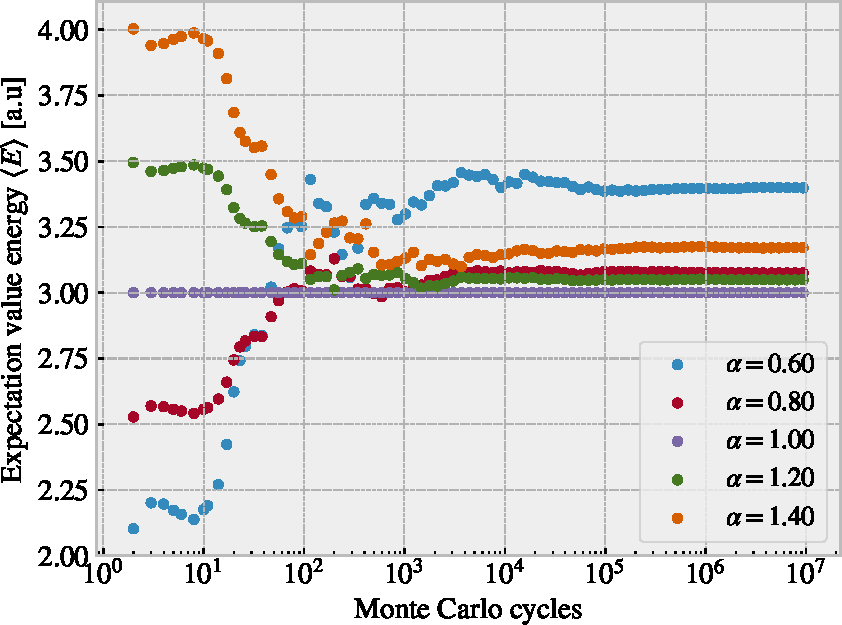
\includegraphics[width=0.485\textwidth]{../figures/stability_energy_E0.pdf}
  \caption{The expectation value of the energy is displayed as a function of the number of Monte Carlo cycles. We have done this for different values of the variational parameter $\alpha$ for the noninteracting Hamiltonian with $\Psi_{T1}$ as trial wave function. This is displayed to study the stabilization and equilibration time of the Metropolis algorithm, and it's dependence on the variational parameter $\alpha$. We observe the lowest energy, and an instantaneous stabilization, for $\alpha=1.00$, while all other values produce a larger energy.}
  \label{fig:stability_energy_E0}
\end{figure}

\begin{figure}
  \centering
  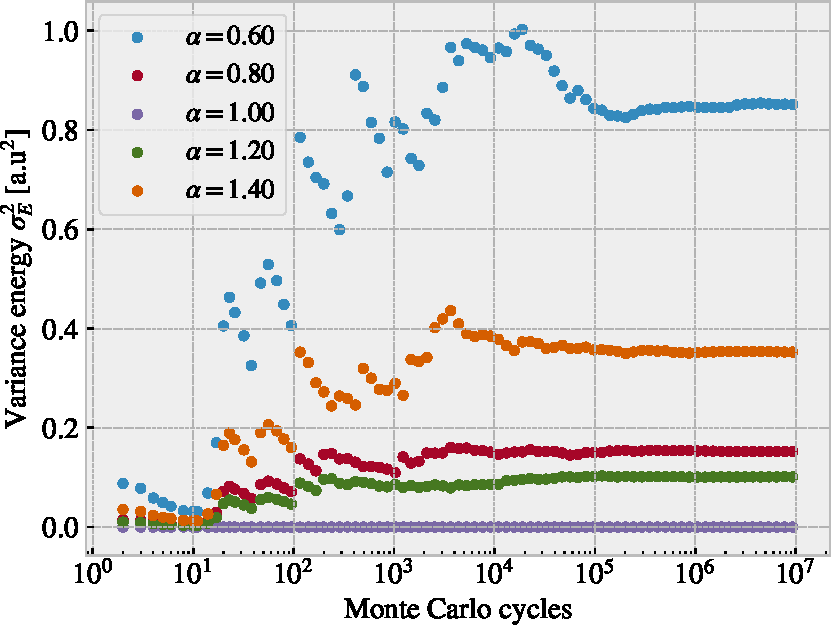
\includegraphics[width=0.485\textwidth]{../figures/stability_variance_E0.pdf}
  \caption{The variance in energy is displayed as a function of the number of Monte Carlo cycles. This is done for different values of the variational parameter $\alpha$ in the noninteracting case, using $\Psi_{T1}$ as trial wave function. This is displayed to study the stabilization and equilibration time of the Metropolis algorithm, and it's dependence on the variational parameter $\alpha$. We observe a variance of $0$, and an instantaneous stabilization, for $\alpha=1.00$, while all other values produce a larger variance, with a longer stabilization.}
  \label{fig:stability_variance_E0}
\end{figure}

\begin{figure}
  \centering
  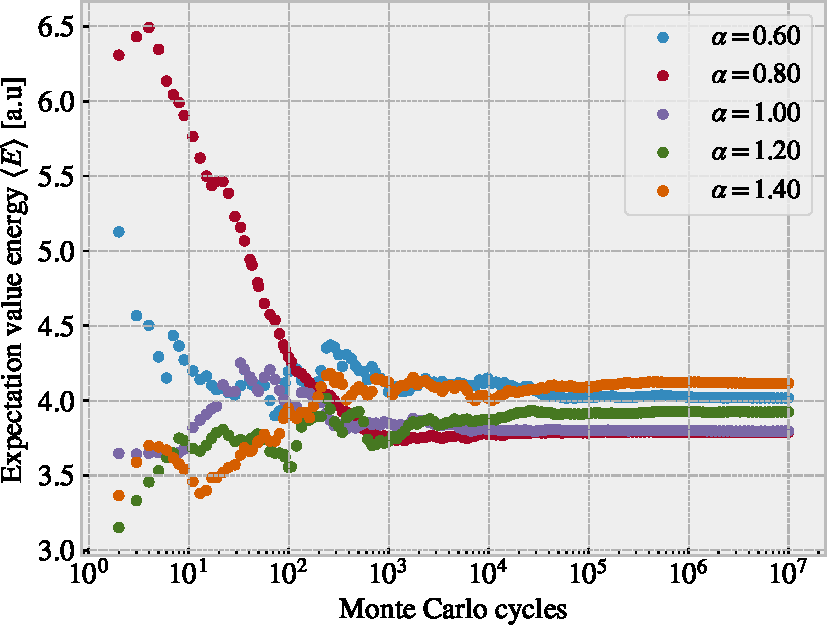
\includegraphics[width=0.485\textwidth]{../figures/stability_energy_E1.pdf}
  \caption{The expectation value of the energy is displayed as a function of the number of Monte Carlo cycles for different values of the variational parameter $\alpha$. This is done for the interacting Hamiltonian, using $\Psi_{T1}$ as trial wave function. This is displayed to study the stabilization and equilibration time of the Metropolis algorithm, and it's dependence on the variational parameter $\alpha$, when we include the electron-electron repulsion in our Hamiltonian. None of the values used for $\alpha$ gives an assertive lowest energy, and they all stabilize after around $10^5$ Monte Carlo cycles.}
  \label{fig:stability_energy_E1}
\end{figure}

\begin{figure}
  \centering
  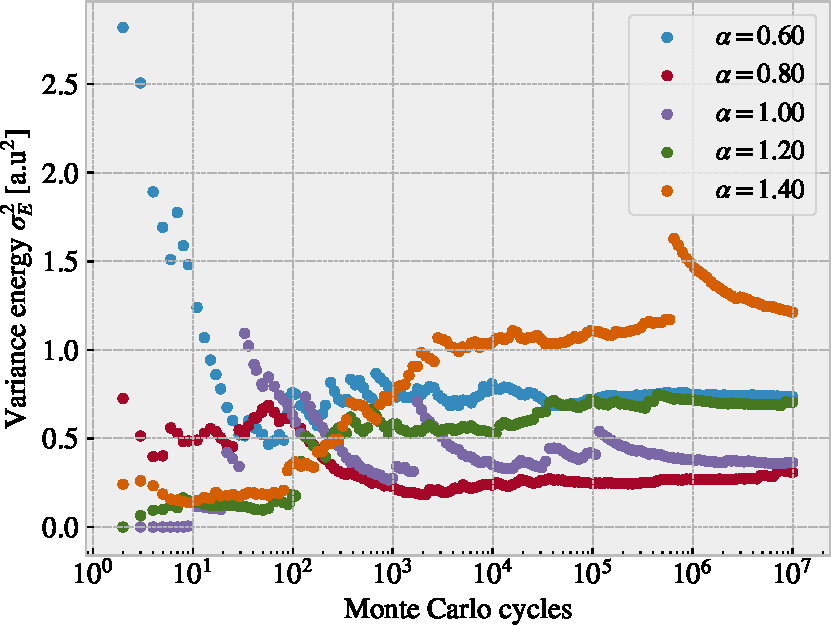
\includegraphics[width=0.485\textwidth]{../figures/stability_variance_E1.pdf}
  \caption{The variance in the energy is displayed as a function of the number of Monte Carlo cycles for different values of the variational parameter $\alpha$. We have used the interacting Hamiltonian with $\Psi_{T1}$ as trial wave function. This is displayed to study the stabilization and equilibration time of the Metropolis algorithm, and it's dependence on the variational parameter $\alpha$, when we include the electron-electron repulsion in our Hamiltonian. The variance behaves differently compared to the noninteracting Hamiltonian, where we now observe sudden jumps, and the equilibration time is harder to estimate. None of the values used for $\alpha$ result in zero variance.}
  \label{fig:stability_variance_E1}
\end{figure}

\subsection{Finding the optimal step length}
In Fig. \vref{fig:acceptence_rate} the acceptance rate of the trial position vector is displayed as a function of the step length $\delta$, using $\Psi_{T1}$ with the noninteracting Hamiltonian. The intersection for each $\alpha$-line with the $50\%$ value is then calculated to find the ideal value of $\delta$. The ideal step length $\delta$ is shown as a function of $\alpha$ in Fig. \vref{fig:ideal_step}. We use this best-fit line to calculate the ideal step length as a function of $\alpha$ in all of our results.
The best fit curve is found to be $\delta(\alpha)=\,1.39(3)\,\times\,\alpha^{-0.50(1)}$, which is approximately
\begin{equation}
  \delta(\alpha) = \frac{1.39}{\sqrt{\alpha}}.
\end{equation}

\begin{figure}
  \centering
  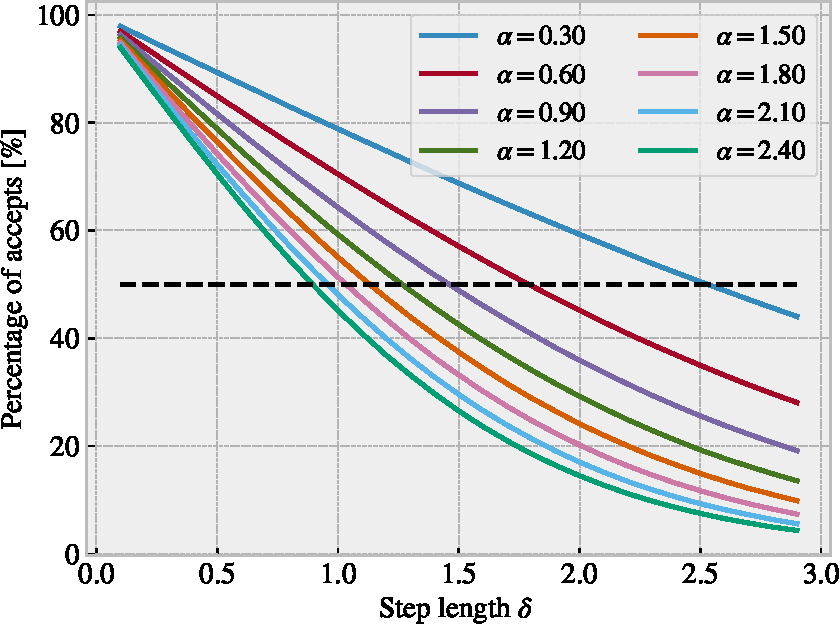
\includegraphics[width=0.485\textwidth]{../figures/acceptence_rate.pdf}
  \caption{The acceptance rate for different values of $\alpha$ is displayed as a function of the step length $\delta$. The black horizontal line displays the ideal value of the acceptance rate, $50\%$. The intersections with this line is used to calculate the ideal value of $\delta$ as a function of $\alpha$. The intervals of step lengths is such that we go from an acceptance rate of close $100\%$ to almost $0\%$ depending on $\alpha$. The calculations were done for the noninteracting Hamilton using $\Psi_{T1}$, and was done for more $\alpha$ values than displayed in this figure.}
  \label{fig:acceptence_rate}
\end{figure}

\begin{figure}
  \centering
  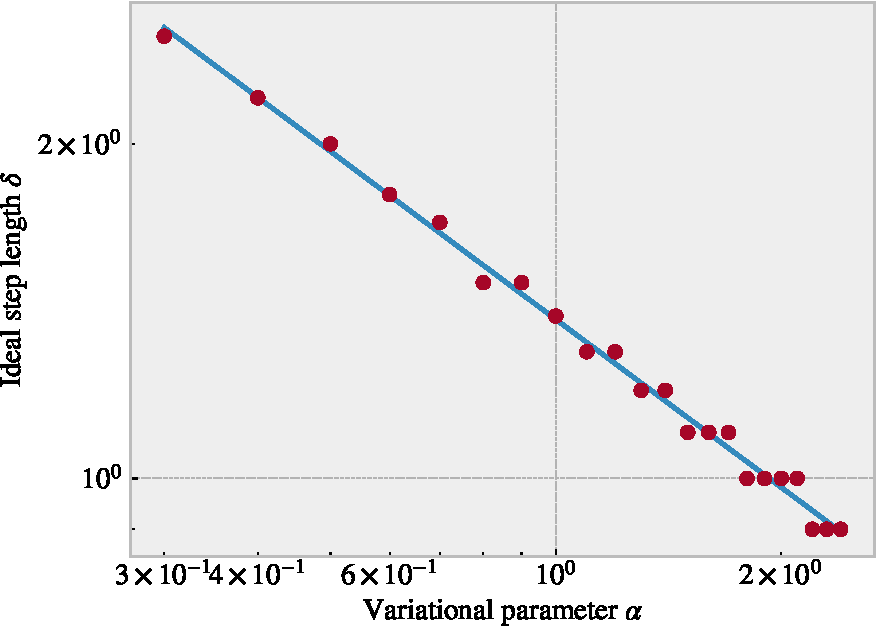
\includegraphics[width=0.485\textwidth]{../figures/ideal_step.pdf}
  \caption{The step length $\delta$ resulting in a $50\%$ acceptance rate is shown as a function of the variational parameter $\alpha$. The values were calculated from the intersection with the $50\%$ line displayed in Fig. \vref{fig:acceptence_rate}. The calculations were done for the noninteracting Hamiltonian using the trial wave function $\Psi_{T1}$. The best fite line is calculated through the least squares method \cite{squires} giving us $\delta(\alpha) \approx 1.39/\sqrt{\alpha}$, which is used throughout our calculations.}
  \label{fig:ideal_step}
\end{figure}

\subsection{The first trial wave function $\boldsymbol{\Psi_{T1}}$}
The energy for the noninteracting electrons using trial wave function $\Psi_{T1}$ is displayed as a function of the variational parameter $\alpha$ in Fig. \vref{fig:energy_E0}, and the variance in energy is displayed in Fig. \vref{fig:variance_E0}. It is displayed together with the energy and variance using the same trial wave function, but including the electron-electron interaction in the Hamiltonian. The value of $\alpha$ resulting in the minimal value in energy and variance for the noninteracting case is $\alpha=1.00(1)$. Giving an energy of $3.00(0)$ a.u, with zero variance.
For the interacting case the optimal value is $\alpha=0.87(1)$, resulting in an energy of $3.77(2)$ a.u, with a variance of $0.28$ a.u$^2$.\par


\begin{figure}
  \centering
  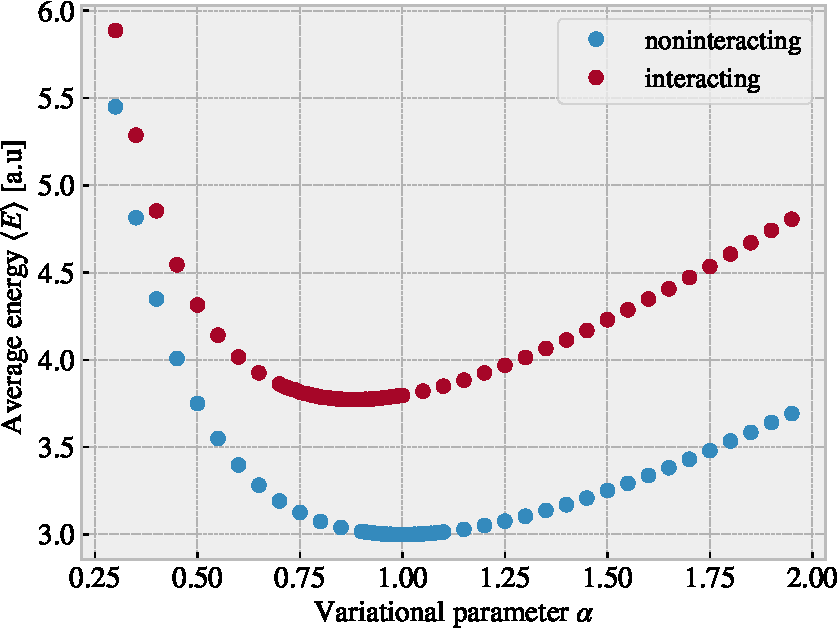
\includegraphics[width=0.485\textwidth]{../figures/energy_c.pdf}
  \caption{The expectation value of the energy is displayed as a function of the variational parameter $\alpha$ for the noninteracting and interacting Hamiltonian using the trial wave function $\Psi_{T1}$. This was calculated using $10^8$ MC cycles, with a step size for $\alpha$ equal to $0.05$, which was decreased to $0.01$ around the minima. The optimal value of $\alpha$ is the one corresponding to the minimal energy, which was found to be $1.00(1)$ for the noninteracting Hamiltonian, and $0.87(1)$ for the interacting Hamiltonian.}
  \label{fig:energy_E0}
\end{figure}

\begin{figure}
  \centering
  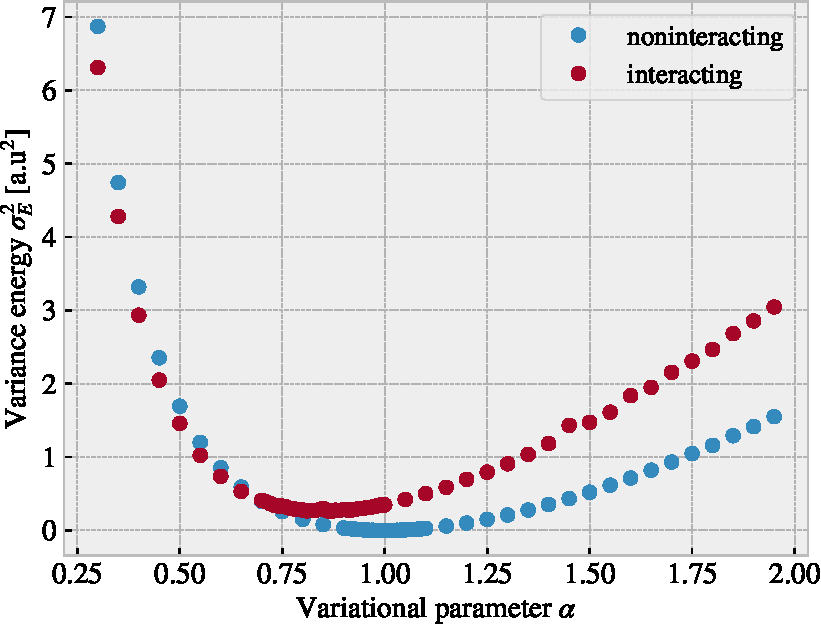
\includegraphics[width=0.485\textwidth]{../figures/variance_c.pdf}
  \caption{The variance of the energy is displayed as a function of the variational parameter $\alpha$ for the noninteracting and interacting Hamiltonian using the trial wave function $\Psi_{T1}$. This was calculated using $10^8$ MC cycles, with a step size for $\alpha$ equal to $0.05$, which was decreased to $0.01$ around the minima. The optimal value of $\alpha$ is the one corresponding to the minimal variance, which was found to be $1.00(1)$ for the noninteracting Hamiltonian, and $0.87(1)$ for the interacting Hamiltonian. These values are consistent with what we observed for the minimal energy, displayed in Fig. \vref{fig:energy_E0}.}
  \label{fig:variance_E0}
\end{figure}

These optimal values of $\alpha$ are used to compute the average distance between the two electrons for different values of the characteristic frequency $\omega$ of the harmonic oscillator, for the interacting and noninteracting case. The resulting expectation values of the distance are displayed in Table \vref{table:omega_1}.

\begin{table}[]
  \caption{The expectation value of the distance between the two electrons is displayed for different characteristic frequencies of the oscillator potential $\omega$ for the interacting and noninteracting Hamiltonian using the trial wave function $\Psi_{T1}$. We see a decrease in the expectation value of the distance as we increase the frequency of the oscillator potential. In addition we notice that the electrons are further apart when we include the interaction in the Hamiltonian. To achieve these values we used the optimal value of $\alpha$ found earlier, $\alpha=1.00$ for noninteracting, and $\alpha=0.87$ for the interacting Hamiltonian, with $10^{8}$ Monte Carlo cycles. The uncertainties are calculated from the standard deviation of the expectation values.}
  \begin{tabular}{@{}ccc@{}}
  \toprule
  $\quad\omega\quad$ & $\quad\langle r_{12} \rangle$ noninteracting $\quad$ & $\quad\langle r_{12} \rangle$ interacting $\quad$\\ \midrule
  0.01 & 15.92(2) & 16.90(1) \\
  0.50 & 2.256(1) & 2.417(1) \\
  1.00 & 1.595(1) & 1.711(1) \\ \botrule
  \end{tabular}
  \label{table:omega_1}
\end{table}

\subsection{The second trial wave function $\boldsymbol{\Psi_{T2}}$}

The expectation value of the energy in the interacting case is calculated to find the optimal values of $\alpha$ and $\beta$  using $\Psi_{T2}$ as the trial wave function. This is done for a grid for different combinations of $\alpha$ and $\beta$. The resulting energies are shown in Fig. \vref{fig:3D}. With this data we found that the optimal combination is $\alpha=0.995(5)$ and $\beta=0.280(5)$, giving an energy of $3.7302(5)$ a.u. The uncertainties in $\alpha$ and $\beta$ come from the resolution of the grid, while the uncertainty in the energy is from the standard deviation of the sampled expectation values. \par

\begin{figure}
  \centering
  
\includegraphics[width=0.485\textwidth]{../figures/3D.pdf}
  \caption{The expectation value of the energy is displayed as a function of the two variational parameters $\alpha$ and $\beta$ for the interacting Hamiltonian using the trial wave function $\Psi_{T2}$. This was calculated with a step size for both $\alpha$ and $\beta$ equal to $0.005$ for the whole grid, with $10^8$ Monte Carlo cycles. The optimal value for $\alpha$ and $\beta$ were fond to be $\alpha=0.995(5)$ and $\beta=0.280(5)$ respectively, resulting in an energy of $3.7302(5)$ a.u. The uncertainties in $\alpha$ and $\beta$ come from the resolution of the grid, while the uncertainty in the energy is from the standard deviation of the sampled expectation values.}
  \label{fig:3D}
\end{figure}

These optimal values of $\alpha$ and $\beta$ are used to calculate the expectation value of the energy and mean distance between the electrons, for different values of the characteristic frequency $\omega$. The expectation value of the energy is compared to the analytical result produced by M. Taut \cite{taut}. This is shown in Table \vref{table:omega_2}.

\begin{table}[]
    \caption{The expectation value of the energy and the distance between the two electrons is displayed for different characteristic frequencies $\omega$ of the oscillator potential, using the trial wave function $\Psi_{T2}$ and the interacting Hamiltonian. To achieve these values we used the optimal value of $\alpha$ and $\beta$ found for each case, $\alpha=0.995$ and $\beta=0.280$ with $10^{8}$ Monte Carlo cycles. The value for $E$ is the analytical energy found by M. Taut \cite{taut}. We observe an increase in the energy as $\omega$ increases. In addition the expectation value of the electrons distance from each other becomes smaller as $\omega$ increases. The upper bound of the energy is close to the analytical energy, while always being greater. The uncertainty in the values are calculated from the standard deviation of the expectation values.}
  \begin{tabular}{@{}ccccc@{}}
  \toprule
$\quad\omega\quad$ & $\quad\langle E \rangle$ [a.u]$ \quad$ & $\sigma_E^2$[a.u$^2$] & $\quad E$[a.u]
& $\qquad\langle r_{12} \rangle\qquad$ \\ \midrule
  0.01     & 0.10(1)  & 0.00076 &   -      & 17.61(3)     \\
  0.0365   & 0.23(1)  & 0.00170 &  0.219   & 9.59(2)      \\
  0.10     & 0.51(2)  & 0.00266 &  0.500   & 5.87(1)      \\
  0.50     & 2.01(6)  & 0.00406 &  2.000   & 2.60(1)      \\
  1.00     & 3.73(1)  & 0.00812 &  3.558       & 1.81(1)  \\ \botrule
  \end{tabular}
  \label{table:omega_2}
\end{table}

\subsection{The virial theorem}
The virial theorem is tested by comparing the total kinetic and potential energy for the interacting and noninteracting Hamiltonians. The result is shown in Fig. \vref{fig:virial}, where $\Psi_{T1}$ with $\alpha=1.00$ is used for the noninteracting Hamiltonian, and $\Psi_{T2}$ is used for the interacting Hamiltonian, with $\alpha=0.995$ and $\beta=0.280$. The contribution from each part of the potential energy is displayed relative to the kinetic energy as a function of the characteristic frequency $\omega$ in Fig. \vref{fig:H0_vs_C}.

\begin{figure}
  \centering
  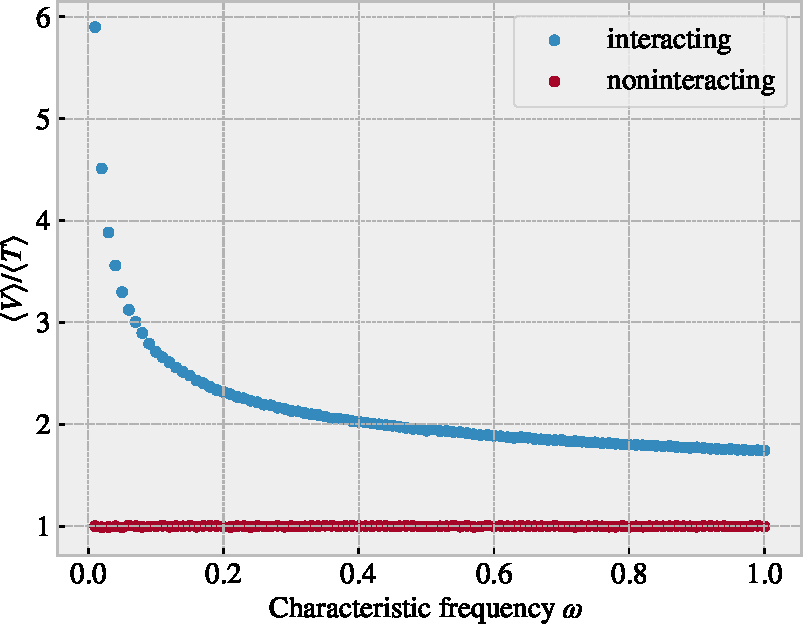
\includegraphics[width=0.485\textwidth]{../figures/virial.pdf}
  \caption{The expectation value of the potential energy divided by the expectation value of the kinetic energy is shown as a function of the characteristic frequency of the oscillator $\omega$ for the interacting and noninteracting Hamiltonians. This is calculated using $\Psi_{T1}$ for the noninteracting case, with $\alpha=1.00$, and $\Psi_{T2}$ for the interacting case, with $\alpha=0.995$ and $\beta=0.280$ with $10^{8}$ Monte Carlo cycles. We observe that the relationship is independent of $\omega$, and always equal to $1$, for the noninteracting Hamiltonian. The relationship is decreasing as $\omega$ increases for the interacting Hamiltonian, always being larger than for the noninteracting Hamiltonian.}
  \label{fig:virial}
\end{figure}


\begin{figure}
  \centering
  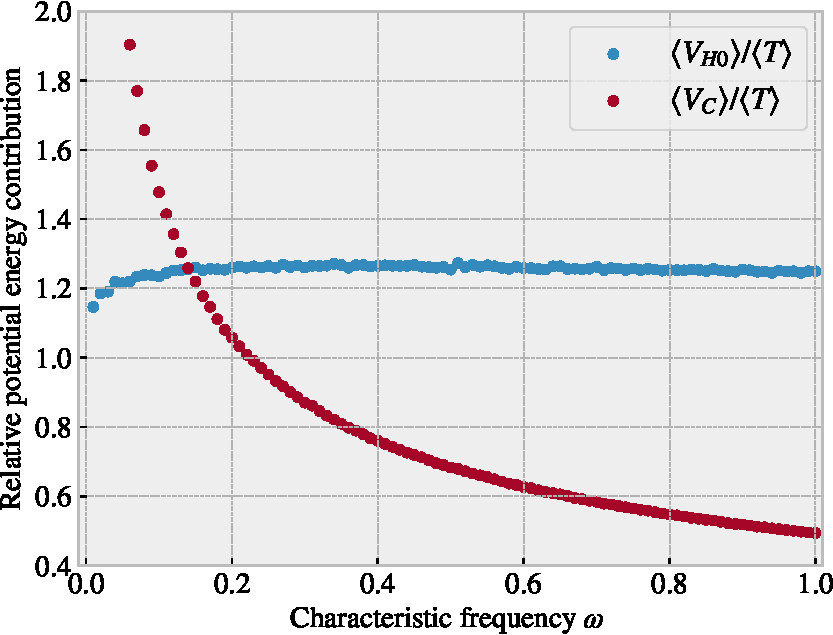
\includegraphics[width=0.485\textwidth]{../figures/H0_vs_C.pdf}
  \caption{The expectation value of the potential energy contribution from the harmonic oscillator (HO) and Coulomb repulsion (C) is displayed relative to the expectation value of the kinetic energy as a function of the characteristic frequency $\omega$ of the oscillator. This is calculated using $\Psi_{T2}$ as the trial wave function with the optimal values for the variational parameters, $\alpha=0.995$ and $\beta=0.280$, and an interacting Hamiltonian with $10^{8}$ Monte Carlo cycles. We observe the harmonic oscillator term being approximately constant for different values of $\omega$, while the potential energy resulting from the Coulomb interaction is decreasing relative to the kinetic energy.}
  \label{fig:H0_vs_C}
\end{figure}


\section{Discussion}

\subsection{Equilibration and benchmarking}
In Fig. \vref{fig:stability_energy_E0} the path to equilibrium is displayed for the energy, for different values of $\alpha$ using $\Psi_{T1}$ without the electron-electron interaction in the Hamiltonian. We see that the for the correct value of $ \alpha$ the exact energy is reached instantaneously, this is not surprising as for $\alpha=1$ the local energy (Eq. \eqref{energy_0}) is always equal to $3\hbar\omega$.\par
We notice that for other values of $\alpha$ the expectation value has to equilibrate before it stabilizes. The further away $\alpha$ is from $1$, the more MC cycles it requires to equilibrate. For these values we see that $10^5$ MC cycles is enough to equilibrate the energy. In our other result we used this many MC cycles to equilibrate the energy before starting sampling the expectation values.

A similar story is told in Fig. \vref{fig:stability_variance_E0}, where the variance is shown as a function of MC cycles using $\Psi_{T1}$ without the electron-electron interaction in the Hamiltonian. We again see that the exact solution with $\alpha=1$ reaches equilibrium immediately, with zero variance. And the deviation from $0$ increases as $\alpha$ is further away from $1$. Again $10^5$ MC cycles are needed to reach equilibrium approximately.

Because the energy equals $3$ a.u with zero variance for $\alpha = 1$, we have benchmarked our algorithm. As explained, $\alpha = 1$ gives the exact analytical solution of the non-interacting system, and thus we expect an energy of $3$ a.u with zero variance.

By taking the electron-electron interaction into account, with the same trial wave function, we produce the results shown in Figs. \ref{fig:stability_energy_E1} and \vref{fig:stability_variance_E1} for the energy and variance respectively. The energy stabilization is quite similar to what we observed without the electron-electron interaction. It stabilizes after $10^5$ MC cycles, with some small jumps after it's equilibration.

We observe that taking the electron-electron interaction into accounts increases the energy by around $0.75$ a.u. Both $\alpha=0.80$ and $\alpha=1.00$  give approximately the same energy, indicating that the change in Hamiltonian changed the ideal value of $\alpha$ as well. The variance shown in Fig. \vref{fig:stability_variance_E1}, on the other hand, tells a completely different story.
Here we observe sudden jumps in the variance, making the variance discontinuous. When we study this closer we see that the reason for the jumps in variance are sudden jumps in the energy. The reason we notice the jumps more clearly in the variance is that it scales as $E^2$, making the jumps more noticeable. When we study the Monte Carlo cycle of the jumps together with the distance $r_{12}$ between the electrons, we see that the jumps in energy are at the exact same instance as the electrons are close to each other. The trial wave function we use does not include the electron-electron repulsion in it's probability density. And as we are using the the trial wave function to sample different positions we will eventually sample a position with the two electrons close to one another. As our Hamiltonian now takes the repulsion into account with the term $1/r_{12}$ the energy will suddenly jump. As the cusp condition is not satisfied for $\Psi_{T1}$, the divergence will not cancel. This is what we observe, where the energy of a state can go from $3$ a.u to $300$ a.u in one step. The trial wave function $\Psi_{T1}$ is therefore not suitable for representing the interacting electrons, as it does not take the repulsion into account and does not satisfy the cusp condition, and this effects the expectation value and variance of the energy.


\subsection{The optimal step length}
From Figs. \ref{fig:acceptence_rate} and \vref{fig:ideal_step} we were able to find the ideal step length as a function of $\alpha$, where we found that the value of $\delta$, resulting in a $50\%$ acceptance rate, is $\delta(\alpha)=1.39/\sqrt{\alpha}$.

From Fig. \ref{fig:acceptence_rate} we see that a too small step length will result in a high acceptance rate, as the change in the probability density will always be close to $0$, making $w$ in our algorithm approximately $1$. For too large step lengths the trial position will move too far away from the origin, making the probability density for the trial position very small compared to the current, and the position will almost never change. We have to find the sweet spot, where we accept the trial position $50\%$ of the time. As the trial wave function used in this plot relates to $\alpha$ through $e^{-\alpha}$ the change in probability density for different positions for larger $\alpha$'s is much larger, and for small $\alpha$'s are much smaller. This explains the acceptance rate displayed in Fig \ref{fig:ideal_step}, where the ideal step decreases as $\alpha$ increases.

\subsection{The first trial wave function $\boldsymbol{\Psi_{T1}}$}

By calculating the average of the expectation values only after reaching equilibrium we produce the results shown in Figs. \ref{fig:energy_E0} and \vref{fig:variance_E0}.
From these two figures we see that for the noninteracting case we were able to reproduce the analytical energy of $3$ a.u, and this energy gives us a variance of $0$, as we should expect when we are using the analytic ground state wave function. For the interacting case we observe a higher energy of $3.77(2)$ a.u. This is because we added a new term in our Hamiltonian, which is always positive. This new term will then increase the energy, as well as pushing the electrons further from the origin; increasing their potential energy from the harmonic oscillator. We can see that we are not working with the true ground state wave function, as we find a minimal variance of $0.28$ a.u$^2$. As the trial wave function used does not take the electron-electron interaction into account it is not surprising that we are not using the true ground state wave function.

\subsection{Average distance}
In Table \ref{table:omega_1} and \vref{table:omega_2} the expectation value of distance between the two electrons is displayed for different values of the characteristic frequency $\omega$. This is displayed for the trial wave function $\Psi_{T1}$ with and without the interacting Hamiltonian, and for $\Psi_{T2}$ with the interacting Hamiltonian. For all cases we observe that the electrons are further apart when $\omega$ decreases. This is because the potential is proportional to $\omega r^2$. From this we see that decreasing $\omega$ makes the potential weaker, making it more probable for the electrons to be further away from the origin.\par
In addition we observe that for every value of $\omega$ the interacting electrons are further apart than the noninteracting electrons. As the electrons are repelling each other we should expect that their distance is larger by including this interaction.\par
One might wonder why the same trial wave function, $\Psi_{T1}$ will force the electrons further apart when we change the Hamiltonian, as we are using the same probability density for our sampling. The reason is that when we include the interaction in the Hamiltonian the ideal value of $\alpha$ changes from $1.00$ to $0.89$. When $\alpha$ is $0.89$, the \textit{steepness} of the probability density of the trial wave function is smaller, and the expectation value of the electrons are further apart. The same trial wave function can therefore take the electron-electron repulsion into account only by altering the variational parameter. By comparing the expectation value of the distance when using $\Psi_{T1}$ and $\Psi_{T2}$ for the interacting Hamiltonian we see that $\Psi_{T2}$ forces the electrons further away from each other. This is because $\Psi_{T2}$ takes the repulsion into the account by weighting the probabilities of the electrons being further apart higher than them being close in the trial wave function.

\subsection{Comparing the trial wave functions}

To get a better estimate of the energy we increase the complexity of our trial wave function to $\Psi_{T2}$, making it a function of two variational parameters; $\alpha$ and $\beta$. We start by minimizing the energy with respect to both parameters, this is shown in Fig. \vref{fig:3D}. This plot shows us that $\Psi_{T2}$ is able to give an energy which is lower than the lowest energy we can get from $\Psi_{T1}$, where we found an energy of $3.77(2)$ a.u using $\Psi_{T1}$ and $3.7302(5)$ a.u using $\Psi_{T2}$. Thus, by using $\Psi_{T2}$ for the optimal values of $\alpha$ and $\beta$, we're able to give a better upper estimate of the ground state energy of the perturbed system than we're able to with $\Psi_{T1}$.
This tells us that $\Psi_{T2}$ with optimal values of $\alpha$ and $\beta$ is a better description of the ground state than $\Psi_{T1}$ with optimal $\alpha$ is. This is what we expect, as $\Psi_{T2}$ have a more realistic description of the repulsion between the two electrons.
As the energy produced by $\Psi_{T2}$ is more accurate than what we computed with $\Psi_{T1}$, we believe that the expectation values of the distance shown in Table \vref{table:omega_2}, computed using $\Psi_{T2}$ is more accurate than what we calculated with $\Psi_{T1}$.

We see from Table \ref{table:omega_2} that the energies obtained by $\Psi_{T2}$ are always slightly bigger than the analytical results of M. Taut \citep{taut}. It is good that our results not are smaller than the analytical values, as that would contradict with the variational method, Eq. \eqref{eq:variational_method}. Also, as the computed energies are not very far off the analytical values, we expect $\Psi_{T2}$ to be close to the form of the ground state of the interacting system, but still not the true ground state.

\subsection{The virial theorem}

From Fig. \ref{fig:virial} we see that the kinetic and potential energies always are equal in the case where the two electrons are not interacting. This is as expected, as the potential then is a pure harmonic oscillator potential and the trial wave function with $\alpha = 1$ is the true ground state. As mentioned in Sec. \ref{sec:virial}, the kinetic and potential energies should be equal in this case.

For the case where the two electrons are interacting, this is not the case any more. First of all, we should not expect the kinetic and potential energy to be equal in the interacting case, as the potential not is a pure $r^{1+1}$ potential any more. We have added a term going as $r^{-1}$, i.e. $n = -2$ in Eq. \ref{eq:general_virial}, and this will affect the virial theorem.

We see that the relation between the potential and kinetic energy is dependent on the value of $\omega$. We believe that this must be a consequence of the two terms in the potential energy contributing differently for different $\omega$'s, i.e. for some $\omega$'s the contribution from the Coulomb interaction to the potential energy is bigger than the harmonic oscillator contribution, and for other $\omega$'s it may be the other way around. Therefore, we calculated the two contributions, so that we could study which of the terms that contributes the most to the potential energy. We see from Fig. \ref{fig:H0_vs_C} that for low $\omega$'s the Coulomb term is dominating, but this term decrease rapidly as $\omega$ increases. The contribution from the harmonic oscillator term is on the other hand almost constant for all $\omega$'s.

We would expect $\ev{T} = -1/2 \ev{V}$ for the Coulomb potential. Added to the harmonic oscillator contribution, the value of $\ev{V}/\ev{T}$ would increase. We see from Fig. \ref{fig:H0_vs_C} that this quotient indeed increases when the contribution from the Coulomb potential is larger than the contribution from the harmonic oscillator potential. We also see that the quotient decreases as the contribution from the Coulomb potential decreases. The quotient never becomes $1$ as we have some contribution from the Coulomb potential, which increases the quotient according to the virial theorem. Also, we do not use a true eigenstate of the system, which may affect the results of the virial theorem.



\section{Conclusion}

We have used the Monte Carlo based Metropolis algorithm together with the variational method to study the ground state of two interacting electrons in a three dimensional harmonic oscillator potential.

We began by studying the equilibration and acceptance rate of the Metropolis algorithm. Using the first trial wave function $\Psi_{T1}$ we found that $10^5$ Monte Carlo cycles were needed to reach equilibrium, for both the interacting and noninteracting Hamiltonian. For the interacting Hamiltonian we observed sudden jumps in the energy and variance, which stems from the fact that the electrons were allowed to be close to one another, with this trial wave function, which did not satisfy the cusp condition, indicating it's flaws for the interacting Hamiltonian. Studying the acceptance of the trial position as a function of the step length $\delta$ we found a best-fit function for the step length $\delta = 1.39/\sqrt{\alpha}$, resulting in a $50\%$ acceptance rate.

The algorithm was tested for the noninteracting case, which had an analytical solution, and we are able to reproduce the analytical ground state energy. We continued by studying the ground state energy with two different trial wave functions, one taking the electron-electron interaction into account, $\Psi_{T2}$, and one which did not, $\Psi_{T1}$. The energies of each wave function were minimized with respect to their variational parameters. We found that the trial wave function taking the interaction into account produces the better upper bound for the ground state energy, $3.702(5)$ a.u, compared to the analytical value of $3.558$ a.u \cite{Hjorten}.

The mean distance between the two electrons increased as the characteristic frequency of the potential was decreased, where the interacting electrons always were further apart, with a larger energy.

The virial theorem was then tested for the interacting and noninteracting case. We found that the virial theorem for the harmonic oscillator potential was indeed correct without the interaction, $\ev{T} = \ev{V}$. When the interaction was taken into account, we observed that the relation $\ev{V}/\ev{T}$ deviated as a function of $\omega$. We found that the deviation was due to which term of the potential energy that dominated for different $\omega$'s, where the repulsion dominated for small $\omega$, but decreased exponentially as $\omega$ was increased.

\section{Comments}
All of the code used is available on our GitHub\footnote{\url{http://www.github.uio.no/cecilgl/FYS4150}}${}^{,}$\footnote{\url{http://www.github.uio.no/ivarsh/FYS4150}}. Here the \texttt{README.MD} files will describe the structure of our GitHub, and the purpose of each program. The code itself will also include notes explaining what it does.

\section{Acknowledgements}
We want to thank professor Olav Fredrik Syljuåsen for teaching us quantum mechanics, and giving us access to a computer with $64$ cores to speed up our numerical calculations.

\bibliography{citations.bib}
\bibliographystyle{plain}
\newpage
\onecolumngrid
\appendix

\section{Deriving the variational method}\label{sec:appendix}
Given a trial state $\ket{\psi}$ and a known Hamiltonian $\hat{H}$ with unknown eigenstates we calculate the expectation value by
\begin{equation}
  E_{\mathrm{trial}} = \bra{\psi}\hat{H}\ket{\psi}.
\end{equation}
By writing the state as a linear combinations of the unknown eigenstates of $\hat{H}$, denoted $\ket{n}$, with eigenvalue $E_n$ we have
\begin{equation}
  E_{\mathrm{trial}} = \sum_{n}\sum_{m}c_n^{*}\bra{n} \hat{H}\ket{m}c_m.
\end{equation}
We can do this as we know that the eigenstates of Hermitian operators span the Hilbert space, and we can therefore express any function as a linear combination of the eigenstates. As $\ket{n}$ are eigenstates of the Hamiltonian, and orthonormal $\braket{n}{m}=\delta_{m,n}$, we get
\begin{equation}
  E_{\mathrm{trial}} = \sum_n \abs{c_n}^2E_n.
\end{equation}
From definition of the ground state, we know that $E_n$ is greater or equal to the ground state energy
\begin{equation}
  E_{\mathrm{trial}} = \sum_n \abs{c_n}^2E_n \geq \sum_n \abs{c_n}^2E_0  = E_0.
\end{equation}
We see that the we can only get the trial energy to equal the ground state energy if $c_n=\delta_{n,0}$, meaning that our guess of trial wave function was in fact the true ground state wave function.

\section{Local energy $\boldsymbol{\Psi_{T1}}$}\label{sec:appendix_trial_1}

For the case of the non-interacting Hamiltonian (Eq. \eqref{hamil_non_interact}), $\Psi_{T1}$ gives a local energy
\begin{equation}
  E_{L1}(\mathbf{r_1}, \mathbf{r_2}) = \frac{1}{2}\omega^2\left(r_1^2 + r_2^2 \right)\left( 1 - \alpha^2  \right) + 3\alpha \omega.
\end{equation}
This can easily be shown by using the definition of local energy, given in Eq. \eqref{eq:E_local}.
The Laplacian in spherical coordinates is
\begin{equation}
\nabla_1^2 = \frac{1}{r_1^2}\frac{\partial}{\partial r_1}\left(r_1^2\frac{\partial}{\partial r_1}\right)
 + \frac{1}{r_1^2\sin\theta_1}\frac{\partial}{\partial\theta_1}\left(\sin\theta_1 \frac{\partial}{\partial\theta_1}\right)
 + \frac{1}{r_1^2\sin^2\theta_1}\frac{\partial^2}{\partial\phi_1^2}.
\end{equation}
If we let this act on $\Psi_{T1}$, we get
\begin{equation}
\nabla_1^2 \Psi_{T1} = \left(-3\alpha\omega + \alpha^2\omega^2r_1^2\right)\Psi_{T1}.
\end{equation}
Thus, the full local energy becomes
\begin{equation}
\begin{split}
 E_{L1}(\mathbf{r_1}, \mathbf{r_2}) &= \frac{1}{\Psi_{T1}}\left(-\frac{1}{2}\nabla_1^2 - \frac{1}{2}\nabla_2^2 + \frac{1}{2}\omega^2\left(r_1^2 + r_2^2\right)\right)\Psi_{T1}\\
 &= \frac{1}{\Psi_{T1}}\left(-\frac{1}{2}\left(-3\alpha\omega + \alpha^2\omega^2r_1^2\right)\right.
\left. - \frac{1}{2}\left(-3\alpha\omega + \alpha^2\omega^2r_2^2\right) \right.
\left. + \frac{1}{2}\omega^2\left(r_1^2 + r_2^2\right)\right)\Psi_{T1} \\ &=\frac{1}{2}\omega^2\left(r_1^2 + r_2^2 \right)\left( 1 - \alpha^2  \right) + 3\alpha \omega.
\end{split}
\end{equation}
For the interacting Hamiltonian (Eq. \eqref{hamil_interact}), we only get an additional term, so that the local energy becomes
\begin{equation}
  E_{L1}(\mathbf{r_1}, \mathbf{r_2}) = \frac{1}{2}\omega^2\left(r_1^2 + r_2^2 \right)\left( 1 - \alpha^2  \right) + 3\alpha \omega + \frac{1}{r_{12}}.
\end{equation}

\section{Local energy $\boldsymbol{\Psi_{T2}}$}\label{sec:appendix_trial_2}
For the case of the interacting Hamiltonian (Eq. \eqref{hamil_interact}), $\Psi_{T2}$ gives a local energy
\begin{align}
 &E_{L2} = \frac{1}{2}\omega^2\left(r_1^2 + r_2^2 \right)\left( 1 - \alpha^2  \right) + 3\alpha \omega + \frac{1}{r_{12}} + \frac{1}{2\left(1+\beta r_{12}\right)^2}\left(\alpha\omega r_{12} - \frac{1}{2\left(1+\beta r_{12}\right)^2} - \frac{1}{r_{12}}  + \frac{2\beta}{1+\beta r_{12}}\right)
\end{align}
This can not so easily be shown by using the definition of local energy, given in Eq. \eqref{eq:E_local}. Due to the Jastrow factor our trial wave function is
\begin{equation}
    \Psi_{T2}(\mathbf{r_1}, \mathbf{r_2}) = C e^{-\alpha\omega(r_1^2 + r_2^2)/2}\,\cdot\, e^{r_{12}/[2\left( 1 + \beta r_{12} \right)]} = \Psi_{T1}\cdot J(r_{12})
\end{equation}
where $r_{12}$ is $\sqrt{(x_1-x_2)^2 + (y_1-y_2)^2 + (z_1-z_2)^2}$ and $J(r_{12})$ is the Jastrow factor. The potential energy term does not contain any derivatives, and can be calculated easily. The kinetic energy term is more complicated. When taking the double derivative of $\Psi_{T2}$ with respect to the variable $q_i$ we get
\begin{equation}
  \pdv[2]{}{q_i}\left(\Psi_{T1} J\right) = \Psi_{T1}\pdv[2]{J}{q_i} + 2\pdv{\Psi_{T1}}{q_i}\pdv{J}{q_i} + J\pdv[2]{\Psi_{T1}}{q_i}.
\end{equation}
We have already calculated $\partial^2\Psi_{T1}/\partial q_i^2$ as this is what we needed to calculate to find kinetic energy of $\Psi_{T1}$. We need to calculate the two other terms. We begin with the $\partial^2 J/\partial q_i^2$ term. We need to calculate the double derivative of the Jastrow factor, for each coordinate $x_1$, $x_2$, $y_1$, $y_2$, $z_1$ and $z_2$. To reduce the notation we will write $r_{12}$ as just $r$. Let's begin by calculating the double derivative for $x_1$
\begingroup\makeatletter\def\f@size{8.5}\check@mathfonts
\begin{gather}
  \frac{\pdv[2]{}{x_1}e^{\frac{r}{2( 1 + \beta r)}}}{e^{\frac{r}{2( 1 + \beta r)}}} =
  \Bigg( \frac{(x_1-x_2)^2\beta^2}{r(1+\beta r)^3} - \frac{(x_1-x_2)^2}{2r^3(1+\beta r)} - \frac{(x_1-x_2)^2\beta}{2r^2(1+\beta r)^2} +\frac{1}{2r(1+\beta r)}-\frac{\beta}{2(1+\beta r)^2}\Bigg) +\Bigg( \frac{x_1-x_2}{2r(1+\beta r)} - \frac{\beta(x_1-x_2)}{2(1+\beta r)^2}  \Bigg)^2
\end{gather}
\endgroup
We do the same for $x_2$ and find
\begingroup\makeatletter\def\f@size{8.5}\check@mathfonts
\begin{gather}
  \frac{\pdv[2]{}{x_2}e^{\frac{r}{2( 1 + \beta r)}}}{e^{\frac{r}{2( 1 + \beta r)}}} =
  \Bigg( \frac{(x_1-x_2)^2\beta^2}{r(1+\beta r)^3} - \frac{(x_1-x_2)^2}{2r^3(1+\beta r)} - \frac{(x_1-x_2)^2\beta}{2r^2(1+\beta r)^2} +\frac{1}{2r(1+\beta r)}-\frac{\beta}{2(1+\beta r)^2}\Bigg) +\Bigg(\frac{\beta(x_1-x_2)}{2(1+\beta r)^2} - \frac{x_1-x_2}{2r(1+\beta r)} \Bigg)^2
\end{gather}
\endgroup
We see that they give exactly the same expression, except for the sign inside the squared parenthesis, which does not matter as we are squaring it. As the wave function $\Psi_{T2}$ is symmetric with respect to $x$, $y$ and $z$ we do not need to calculate the derivatives for these directly, as they have to be identical to what we just found, only swapping the $x$'s with $y$'s or $z$'s. We save the squared parenthesis for later, and sum over the first parenthesis for the derivatives with respect to $x_1$, $y_1$ and $z_1$, giving us
\begin{align}
  &+ \Bigg( \frac{(x_1-x_2)^2\beta^2}{r(1+\beta r)^3} - \frac{(x_1-x_2)^2}{2r^3(1+\beta r)} - \frac{(x_1-x_2)^2\beta}{2r^2(1+\beta r)^2}  +\frac{1}{2r(1+\beta r)}-\frac{\beta}{2(1+\beta r)^2}\Bigg) \nonumber \\
   &+ \Bigg( \frac{(y_1-y_2)^2\beta^2}{r(1+\beta r)^3} - \frac{(y_1-y_2)^2}{2r^3(1+\beta r)} - \frac{(y_1-y_2)^2\beta}{2r^2(1+\beta r)^2} +\frac{1}{2r(1+\beta r)}-\frac{\beta}{2(1+\beta r)^2}\Bigg)\\
   &+\Bigg( \frac{(z_1-z_2)^2\beta^2}{r(1+\beta r)^3} - \frac{(z_1-z_2)^2}{2r^3(1+\beta r)} - \frac{(z_1-z_2)^2\beta}{2r^2(1+\beta r)^2} +\frac{1}{2r(1+\beta r)}-\frac{\beta}{2(1+\beta r)^2}\Bigg). \nonumber
\end{align}
Adding together the terms with the same denominator, and using the fact that $(x_1-x_2)^2+(y_1-y_2)^2+(z_1-z_2)^2=r^2$, we get
\begin{gather}
  \frac{r^2\beta^2}{r(1+\beta r)^3} - \frac{r^2}{2r^3(1+\beta r)} - \frac{r^2\beta}{2r^2(1+\beta r)^2} +\frac{1}{2r(1+\beta r)}-\frac{\beta}{2(1+\beta r)^2}.
\end{gather}
By cancelling the $r$'s and adding together the common terms we are left with
\begin{gather}
  \frac{r\beta^2}{(1+\beta r)^3} + \frac{1}{r(1+\beta r)} - \frac{2\beta}{(1+\beta r)^2}.
\end{gather}
We extract a common factor
\begin{gather}
  \frac{1}{(1+\beta r)^2}\left( \frac{r\beta^2}{(1+\beta r)} + \frac{1+\beta r}{r} - 2\beta  \right).
\end{gather}
We expand the second term into two terms, and multiply $-2\beta$ by $(1+\beta r)$ in the numerator and denominator, and after the smoke has cleared we have
\begin{gather}
  \frac{1}{(1+\beta r)^2}\left(\frac{1}{r} - \frac{\beta}{1+\beta r} \right).
\end{gather}
We showed earlier that we got the same expression when we calculated the double derivative with respect to the positions of the second electron, with sub index $2$, meaning that for the full expression we need to multiply by $2$, giving us
\begin{gather}
  \frac{2}{(1+\beta r)^2}\left(\frac{1}{r} - \frac{\beta}{1+\beta r} \right). \label{first}
\end{gather}
We have to remember that we completely ignored the squared parenthesis, let's try to simplify this expression as well. For the $x_1$ derivative the square bracket was
\begin{gather}
  \left( \frac{\beta(x_1-x_2)}{2(1+\beta r)^2} - \frac{x_1-x_2}{2r(1+\beta r)} \right)^2 = \frac{\beta^2(x_1-x_2)^2}{4(1+\beta r)^4} + \frac{(x_1-x_2)^2}{4r^2(1+\beta r)^2} - \frac{2\beta(x_1-x_2)^2}{4r(1+\beta r)^3}.
\end{gather}
As the wave function $\Psi_{T2}$ is symmetric with respect to $x$, $y$ and $z$ we see that we would get the exact same expression by taking the double derivative with respect to $y$ or $z$. Adding the terms from $y$ and $z$ we can use that $(x_1-x_2)^2+(y_1-y_2)^2+(z_1-z_2)^2=r^2$, just as before, we get
\begin{gather}
  \frac{\beta^2r^2}{4(1+\beta r)^4} + \frac{r^2}{4r^2(1+\beta r)^2} - \frac{2\beta r^2}{4r(1+\beta r)^3}
\end{gather}
We cancel the $r$'s and pull out a common factor
\begin{gather}
  \frac{1}{4(1+\beta r)^2}\left( \frac{\beta^2r^2}{(1+\beta r)^2} + 1 - \frac{2\beta r}{1+\beta r} \right).
\end{gather}
With every term we multiply the numerator and denominator by the same number which makes every term inside the parenthesis to have the same denominator. Doing this we see that almost everything cancels, and we are left with
\begin{gather}
  \frac{1}{4(1+\beta r)^4} \label{second}.
\end{gather}
As we have the same square parenthesis when calculating the double derivative with respect to the positions of the second electron, with sub index $2$, we need to multiply the expression we just found by $2$ to get the full result.
We will now combine the two terms (\ref{first}, \ref{second}) we had when calculating the double derivative
\begin{gather}
  \frac{1}{2(1+\beta r)^4} + \frac{2}{(1+\beta r)^2}\left(\frac{1}{r} - \frac{\beta}{1+\beta r} \right).
\end{gather}
Using the common factor we can write this as
\begin{gather}
  \frac{1}{(1+\beta r)^2}\left(\frac{2}{r} - \frac{2\beta}{1+\beta r} + \frac{1}{2(1+\beta r)^2}  \right).
\end{gather}
We have now calculated the double derivative of the Jastrow factor. The only term we need to calculate is $\partial \Psi_{T1}/\partial q_i \partial J/ \partial q_i$. We begin by calculating the derivative of $\Psi_{T1}$ with respect to $x_1$
\begin{equation}
  \pdv{}{x_1}\Psi_{T1} = \pdv{}{x_1} C e^{-\alpha\omega/2(x_1^2 + y_1^2 + z_1^2 + x_2^2 + y_2^2 + z_2^2)} = -\alpha \omega x_1 C e^{-\alpha/2(x_1^2 + y_1^2 + z_1^2 + x_2^2 + y_2^2 + z_2^2)} = - \alpha \omega x_1 \Psi_{T1}.
\end{equation}
And we see that we get the exact same result when taking the derivative with respect to $x_2$
\begin{equation}
  \pdv{}{x_2}\Psi_{T1} = \pdv{}{x_2} C e^{-\alpha\omega/2(x_1^2 + y_1^2 + z_1^2 + x_2^2 + y_2^2 + z_2^2)} = -\alpha x_2 C e^{-\alpha\omega/2(x_1^2 + y_1^2 + z_1^2 + x_2^2 + y_2^2 + z_2^2)} = - \alpha\omega x_2 \Psi_{T1}.
\end{equation}
Taking the derivative of the Jastrow factor with respect to $x_1$ gives us
\begin{equation}
  \pdv{}{x_1}J = \left( \frac{x_1-x_2}{2r(\beta r + 1)} - \frac{\beta(x_1-x_2)}{2(\beta r + 1)^2}\right) J.
\end{equation}
And taking the derivative of the Jastrow factor with respect to $x_2$ gives us
\begin{equation}
  \pdv{}{x_2}J = -\left(\frac{x_1-x_2}{2r(\beta r + 1)} - \frac{\beta(x_1-x_2)}{2(\beta r + 1)^2}\right) J.
\end{equation}
Which is the exact same result, but with the opposite sign. What we want to calculate is $\pdv{\Psi_{T1}}{q_i}\pdv{J}{q_i}$, so let's combine the two derivatives for $x_1$
\begin{equation}
  \pdv{\Psi_{T1}}{x_1}\pdv{J}{x_1} = - \alpha\omega x_1 \left( \frac{x_1-x_2}{2r(\beta r + 1)} - \frac{\beta(x_1-x_2)}{2(\beta r + 1)^2}\right) \Psi_{T1} J.
\end{equation}
And do the same for the derivatives with respect to $x_2$
\begin{equation}
  \pdv{\Psi_{T1}}{x_2}\pdv{J}{x_2} = \alpha\omega x_2 \left( \frac{x_1-x_2}{2r(\beta r + 1)} - \frac{\beta(x_1-x_2)}{2(\beta r + 1)^2}\right) \Psi_{T1} J.
\end{equation}
By combining the two we get
\begin{equation}
  \pdv{\Psi_{T1}}{x_2}\pdv{J}{x_2} + \pdv{\Psi_{T1}}{x_1}\pdv{J}{x_1} = - \alpha\omega (x_1-x_2) \left( \frac{x_1-x_2}{2r(\beta r + 1)} - \frac{\beta(x_1-x_2)}{2(\beta r + 1)^2}\right) \Psi_{T1} J.
\end{equation}
We have a common factor $(x_1-x_2)^2$ in each term. Just like earlier we can use that the wave function is symmetric with respect to $x$, $y$ and $z$. Thus, by combining all the six derivatives, and using the fact that $(x_1-x_2)^2+(y_1-y_2)^2+(z_1-z_2)^2=r^2$, we get
\begin{equation}
  - \alpha\omega r^2 \left( \frac{1}{2r(\beta r + 1)} - \frac{\beta}{2(\beta r + 1)^2}\right) \Psi_{T1} J.
\end{equation}
By taking the factor $(1+\beta r)^{-2}$ outside the parenthesis and simplifying the expression inside the parenthesis we are left with
\begin{equation}
 -\frac{r\alpha\omega}{2(1+\beta r)^2}\Psi_{T1}J.
\end{equation}
Now we have calculated all three terms for $(\nabla_1^2 + \nabla_2^2)J\Psi_{T1}$. From this we have the kinetic energy of $\Psi_{T2}$, this has to be combined with the potential energy from the harmonic oscillator. Luckily does the potential terms not contain any differential operators, and we can therefore use the result we found for $\Psi_{T1}$. Combining the calculation we have
\begin{align}
  \frac{1}{\Psi_{T1}J}\hat{H}\left(\Psi_{T1}J\right) &= \left(\frac{1}{2}\omega \left(r_1^2+r_2^2\right)+\frac{1}{r_{12}} -\frac{1}{2}\left( \nabla_1^2 + \nabla_2^2 \right)\right) \Psi_{T1}J \\
  &= E_{L0} +\frac{1}{r} -\frac{1}{2}\left(-\frac{r\alpha\omega}{(1+\beta r)^2} + \frac{1}{(1+\beta r)^2}\left(\frac{2}{r} - \frac{2\beta}{1+\beta r} + \frac{1}{2(1+\beta r)^2}  \right)\right).
\end{align}
Factorizing the common factor outside, and writing $r_{12}$ instead of $r$ we get our final answer for the local energy for $\Psi_{T2}$
\begin{equation}
  E_{L2} = E_{L1} + \frac{1}{2(1+\beta r_{12})^2}\left(r_{12}\alpha\omega - \frac{2}{r_{12}} + \frac{2\beta}{1+\beta r_{12}} - \frac{1}{2(1+\beta r_{12})^2} \right).
\end{equation}
\end{document}
